\documentclass{beamer}
\usepackage{animate}
\usepackage{tikz}
\usepackage{svg}
\usetheme{metropolis}
\begin{document}

\title{Calibration with Machine Learning in Radio Cosmology}
\date{14 November 2023}
\author{Samuel Alan Kossoff Leeney, Harry Bevins, Will Handley, Eloy de Lera Acedo, Jiacong Zhu, Kaan Artuc, Daniel Molnar}
\institute{Machine Learning for Astronomy 2024}
\begin{frame}
  \titlepage
  \begin{tikzpicture}[remember picture, overlay]
    \node[right=4.5cm, above=-4.5cm] at (current page.center)
    {
    
\includegraphics[width=0.3\textwidth]{camlogo.jpg}
    };
    \end{tikzpicture}

  \begin{tikzpicture}[remember picture, overlay]
    \node[right=-4.7cm, above=-4.7cm] at (current page.center)
    {
    
\includegraphics[width=0.25\textwidth]{reach.jpg}
    };
  \end{tikzpicture}

  \begin{tikzpicture}[remember picture, overlay]
    \node[right=1.2cm, above=-4.8cm] at (current page.center)
    {
    
\includegraphics[width=0.15\textwidth]{erc.png}
    };
  \end{tikzpicture}

  \begin{tikzpicture}[remember picture, overlay]
    \node[right=-1.6cm, above=-4.3cm] at (current page.center)
    {
    \includegraphics[width=0.23\textwidth]{ukri.png}
    };
  \end{tikzpicture}
\end{frame}

\begin{frame}{\small{What is calibration in Astronomy?}}
\begin{figure}[h]
  \centering
  \includesvg[width=0.8\textwidth]{whatiscal.svg}
\end{figure}
\vfill
    \tiny{Co-authors: Harry Bevins, Will Handley, Eloy de Lera Acedo, Jiacong Zhu, Kaan Artuc, Daniel Molnar}
  \end{frame}


\begin{frame}{\small{How to calibrate?}}
\begin{figure}[h]
  \centering
  \includesvg[width=0.8\textwidth]{howtocal.svg}
\end{figure}

\vfill
    \tiny{Co-authors: Harry Bevins, Will Handley, Eloy de Lera Acedo, Jiacong Zhu, Kaan Artuc, Daniel Molnar}
  \end{frame}


\begin{frame}{\small{Why is machine learning helpful?}}
\begin{figure}[h]
  \centering
  \includesvg[width=0.7\textwidth]{mlcal.svg}
\end{figure}

\vfill
    \tiny{Co-authors: Harry Bevins, Will Handley, Eloy de Lera Acedo, Jiacong Zhu, Kaan Artuc, Daniel Molnar}
  \end{frame}

\begin{frame}{\small{Machine learning for radiometer calibration in global 21cm cosmology}}
  \begin{figure}
    \centering
    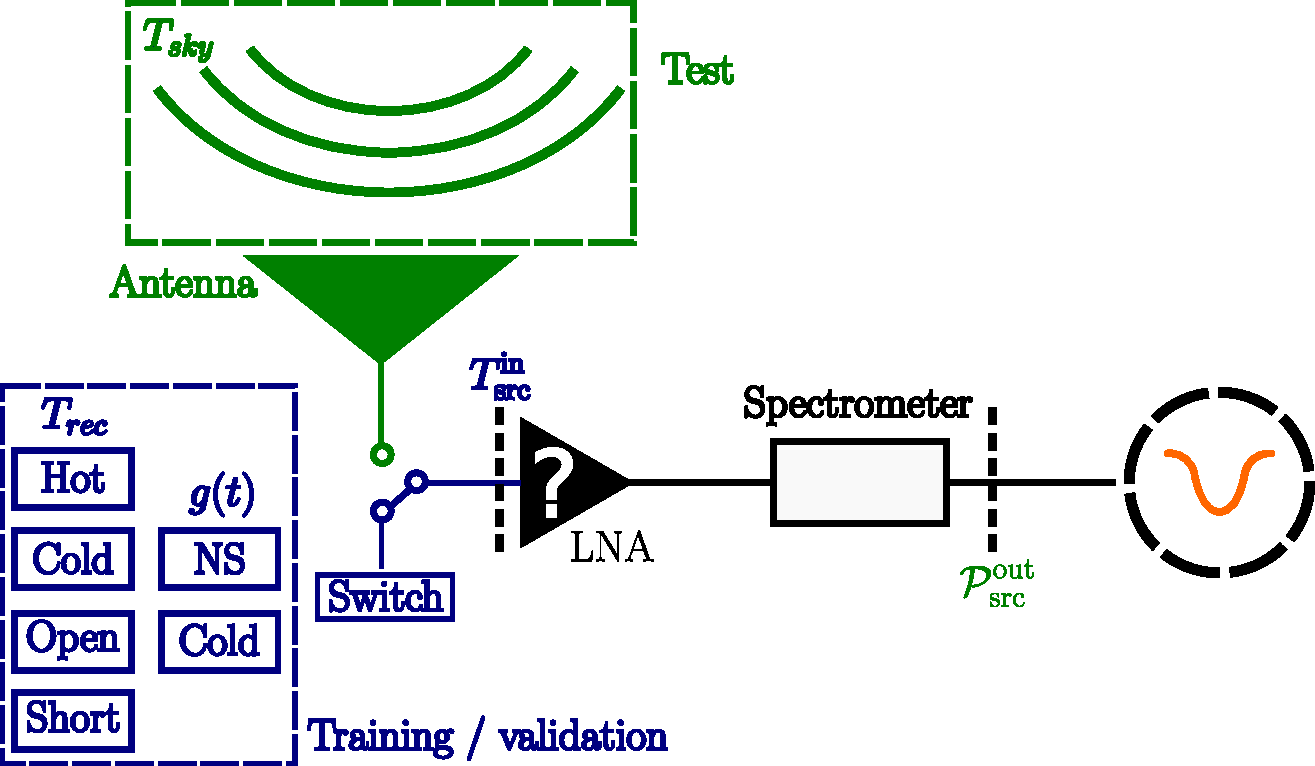
\includegraphics[width=1.05\textwidth]{instrument.pdf}
  \end{figure}
\vfill
    \tiny{Co-authors: Harry Bevins, Will Handley, Eloy de Lera Acedo, Jiacong Zhu, Kaan Artuc, Daniel Molnar}
  \end{frame}

  \begin{frame}{\small{Machine learning for radiometer calibration in global 21cm cosmology}}
    \begin{figure}
    \centering
    \includesvg[width=0.9\textwidth]{nn.svg}
  \end{figure}
\vfill
    \tiny{Co-authors: Harry Bevins, Will Handley, Eloy de Lera Acedo, Jiacong Zhu, Kaan Artuc, Daniel Molnar}

  \end{frame}

  \begin{frame}{\small{Machine learning for radiometer calibration in global 21cm cosmology}}
    \begin{figure}
      \centering
      \includesvg[width=1\textwidth]{results.svg}
    \end{figure}

    \begin{figure}
    \centering
    \includesvg[width=0.3\textwidth]{nn.svg}
  \end{figure}
\vfill
    \tiny{Co-authors: Harry Bevins, Will Handley, Eloy de Lera Acedo, Jiacong Zhu, Kaan Artuc, Daniel Molnar}
  \end{frame}
\end{document}
